% Options for packages loaded elsewhere
% Options for packages loaded elsewhere
\PassOptionsToPackage{unicode}{hyperref}
\PassOptionsToPackage{hyphens}{url}
\PassOptionsToPackage{dvipsnames,svgnames,x11names}{xcolor}
%
\documentclass[
  number]{elsarticle}
\usepackage{xcolor}
\usepackage{amsmath,amssymb}
\setcounter{secnumdepth}{5}
\usepackage{iftex}
\ifPDFTeX
  \usepackage[T1]{fontenc}
  \usepackage[utf8]{inputenc}
  \usepackage{textcomp} % provide euro and other symbols
\else % if luatex or xetex
  \usepackage{unicode-math} % this also loads fontspec
  \defaultfontfeatures{Scale=MatchLowercase}
  \defaultfontfeatures[\rmfamily]{Ligatures=TeX,Scale=1}
\fi
\usepackage{lmodern}
\ifPDFTeX\else
  % xetex/luatex font selection
\fi
% Use upquote if available, for straight quotes in verbatim environments
\IfFileExists{upquote.sty}{\usepackage{upquote}}{}
\IfFileExists{microtype.sty}{% use microtype if available
  \usepackage[]{microtype}
  \UseMicrotypeSet[protrusion]{basicmath} % disable protrusion for tt fonts
}{}
\makeatletter
\@ifundefined{KOMAClassName}{% if non-KOMA class
  \IfFileExists{parskip.sty}{%
    \usepackage{parskip}
  }{% else
    \setlength{\parindent}{0pt}
    \setlength{\parskip}{6pt plus 2pt minus 1pt}}
}{% if KOMA class
  \KOMAoptions{parskip=half}}
\makeatother
% Make \paragraph and \subparagraph free-standing
\makeatletter
\ifx\paragraph\undefined\else
  \let\oldparagraph\paragraph
  \renewcommand{\paragraph}{
    \@ifstar
      \xxxParagraphStar
      \xxxParagraphNoStar
  }
  \newcommand{\xxxParagraphStar}[1]{\oldparagraph*{#1}\mbox{}}
  \newcommand{\xxxParagraphNoStar}[1]{\oldparagraph{#1}\mbox{}}
\fi
\ifx\subparagraph\undefined\else
  \let\oldsubparagraph\subparagraph
  \renewcommand{\subparagraph}{
    \@ifstar
      \xxxSubParagraphStar
      \xxxSubParagraphNoStar
  }
  \newcommand{\xxxSubParagraphStar}[1]{\oldsubparagraph*{#1}\mbox{}}
  \newcommand{\xxxSubParagraphNoStar}[1]{\oldsubparagraph{#1}\mbox{}}
\fi
\makeatother


\usepackage{longtable,booktabs,array}
\usepackage{calc} % for calculating minipage widths
% Correct order of tables after \paragraph or \subparagraph
\usepackage{etoolbox}
\makeatletter
\patchcmd\longtable{\par}{\if@noskipsec\mbox{}\fi\par}{}{}
\makeatother
% Allow footnotes in longtable head/foot
\IfFileExists{footnotehyper.sty}{\usepackage{footnotehyper}}{\usepackage{footnote}}
\makesavenoteenv{longtable}
\usepackage{graphicx}
\makeatletter
\newsavebox\pandoc@box
\newcommand*\pandocbounded[1]{% scales image to fit in text height/width
  \sbox\pandoc@box{#1}%
  \Gscale@div\@tempa{\textheight}{\dimexpr\ht\pandoc@box+\dp\pandoc@box\relax}%
  \Gscale@div\@tempb{\linewidth}{\wd\pandoc@box}%
  \ifdim\@tempb\p@<\@tempa\p@\let\@tempa\@tempb\fi% select the smaller of both
  \ifdim\@tempa\p@<\p@\scalebox{\@tempa}{\usebox\pandoc@box}%
  \else\usebox{\pandoc@box}%
  \fi%
}
% Set default figure placement to htbp
\def\fps@figure{htbp}
\makeatother





\setlength{\emergencystretch}{3em} % prevent overfull lines

\providecommand{\tightlist}{%
  \setlength{\itemsep}{0pt}\setlength{\parskip}{0pt}}



 
\usepackage[]{natbib}
\bibliographystyle{elsarticle-num}


\makeatletter
\@ifpackageloaded{caption}{}{\usepackage{caption}}
\AtBeginDocument{%
\ifdefined\contentsname
  \renewcommand*\contentsname{Table of contents}
\else
  \newcommand\contentsname{Table of contents}
\fi
\ifdefined\listfigurename
  \renewcommand*\listfigurename{List of Figures}
\else
  \newcommand\listfigurename{List of Figures}
\fi
\ifdefined\listtablename
  \renewcommand*\listtablename{List of Tables}
\else
  \newcommand\listtablename{List of Tables}
\fi
\ifdefined\figurename
  \renewcommand*\figurename{Figure}
\else
  \newcommand\figurename{Figure}
\fi
\ifdefined\tablename
  \renewcommand*\tablename{Table}
\else
  \newcommand\tablename{Table}
\fi
}
\@ifpackageloaded{float}{}{\usepackage{float}}
\floatstyle{ruled}
\@ifundefined{c@chapter}{\newfloat{codelisting}{h}{lop}}{\newfloat{codelisting}{h}{lop}[chapter]}
\floatname{codelisting}{Listing}
\newcommand*\listoflistings{\listof{codelisting}{List of Listings}}
\captionsetup{labelsep=period}
\makeatother
\makeatletter
\makeatother
\makeatletter
\@ifpackageloaded{caption}{}{\usepackage{caption}}
\@ifpackageloaded{subcaption}{}{\usepackage{subcaption}}
\makeatother
\usepackage{bookmark}
\IfFileExists{xurl.sty}{\usepackage{xurl}}{} % add URL line breaks if available
\urlstyle{same}
\hypersetup{
  pdftitle={Modeling Response Time: The F \textgreater{} C Phenomenon and the Distance-Difficulty Hypothesis},
  pdfauthor={Nicole Bonge; Ronna C. Turner},
  pdfkeywords={Response Time, Item Response Theory, Multilevel
Modeling, F \textgreater{} C Phenomenon, Distance-Difficulty
Hypothesis},
  colorlinks=true,
  linkcolor={blue},
  filecolor={Maroon},
  citecolor={Blue},
  urlcolor={Blue},
  pdfcreator={LaTeX via pandoc}}


\setlength{\parindent}{6pt}
\begin{document}

\begin{frontmatter}
\title{Modeling Response Time: The F \textgreater{} C Phenomenon and the
Distance-Difficulty Hypothesis}
\author[1]{Nicole Bonge%
\corref{cor1}%
}
 \ead{ngbonge@uark.edu} 
\author[1]{Ronna C. Turner%
%
}
 \ead{rcturner@uark.edu} 

\affiliation[1]{organization={University of Arkansas},,postcodesep={}}

\cortext[cor1]{Corresponding author}


        
\begin{abstract}
Response time has long been thought to be closely related with
intelligence via processing speed. If asked to describe a genius, one
might describe a person who can do complex mental calculations quickly
and with ease. This stereotype that students with high ability level
tend to answer questions fastest has come under question, however, with
research indicating that response time is a complex process, dependent
on more than just ability level. In this study, we use multilevel linear
models to analyze the responses and response times on the 2019 TIMSS
mathematics achievement test for eighth-grade students in the United
States. Our results demonstrate response time's dependency on student
ability level, whether the student answered the item correctly (F
\textgreater{} C phenomenon), and item difficulty in relation to the
student's ability level (distance-difficulty hypothesis). We find
evidence to support the F \textgreater{} C phenomenon, the
distance-difficulty hypothesis, and an interaction between the two. Our
results affirm the complexity of cognitive processes involved in item
responses, and challenge the widespread use of response time as a
stand-alone metric to assess item quality and respondent effort.
\end{abstract}





\begin{keyword}
    Response Time \sep Item Response Theory \sep Multilevel
Modeling \sep F \textgreater{} C Phenomenon \sep 
    Distance-Difficulty Hypothesis
\end{keyword}
\end{frontmatter}
    

\section{Introduction}\label{introduction}

Researchers have long contemplated the role of response time in
achievement testing, and how time-to-completion can inform about an item
functioning and participant performance. Among researchers, it is a
widely held belief that response time is indicative of the cognitive
effort required to answer an item (Höhne et al., 2007), so researchers
use response time to gauge item quality and comprehensibility (Bassili
et al., 1996; Lenzner, 2012; Lenzner et al., 2010), to detect respondent
fatigue (Nguyen, 2017), effort (Bowling et al., 2023; Krosnick, 1991;
Ulitzsch et al., 2022), and other characteristics such as persistence,
motivation, and disengagement (e.g., Nagy \& Ulitzsch, 2021; Wise \&
Demars, 2006). Researchers have also used response time to investigate
other cognitive processes underlying item responses (De Boeck \& Jeon,
2019), with recent research challenging the long-held ``faster equals
smarter'' stereotype (Gernsbacher et al., 2020).

In this study, we extend previous models posed by Tancoš et al.~(2023)
to achievement data, arguing that response time depends on (1) item
difficulty, (2) respondent ability level, (3) the distance between the
item's difficulty and the respondent's ability level (referred to as the
distance-difficulty hypothesis; Thissen, 1983), and (4) whether the
respondent answered the item correctly (F \textgreater{} C phenomenon;
Beckmann, 2000).

\section{Theoretical Framework}\label{theoretical-framework}

\subsection{The F \textgreater{} C Phenomenon}\label{the-f-c-phenomenon}

One approach to modelling response time is the F \textgreater{} C (False
\textgreater{} Correct) phenomenon (Beckmann, 2000), also called the I
\textgreater{} C phenomenon, which posits that respondents take longer
to report incorrect answers than they take to provide correct ones.
Formally, the F \textgreater{} C phenomenon is given by (Beckmann, 2000,
as cited in Tancoš et al., 2023, p.~3):
\begin{equation}\phantomsection\label{eq-FC}{t_{ij} = \mu + \gamma FC_{ij} + \epsilon_{ij},}\end{equation}
where \(t_{ij}\) is the response time of respondent \(j\) on item \(i\);
\(\mu\) is an intercept representing the average response time across
all items and respondents; \(FC_{ij}\) is a binary indicator
representing whether respondent \(j\) answered item \(i\) correctly;
\(\gamma\) is an unstandardized regression coefficient representing the
mean difference in response time between false and correct answers; and
\(\epsilon_{ij}\) is a normally distributed residual.

\subsection{The Distance-Difficulty
Hypothesis}\label{the-distance-difficulty-hypothesis}

Another approach to modeling response time is the distance-difficulty
hypothesis, based in item response theory, proposed originally by
Thissen (1983). The distance-difficulty hypothesis states that response
time decreases with increasing distance between an item's difficulty
(\(b_i\)) and a respondent's ability level (\(\theta_j\)), given by
\(\delta_{ij} = |\theta_j-b_i|\), called person-item distance. In other
words, a respondent should take longer to answer a question that is
close to their ability level. Conversely, a respondent should take less
time to answer a question that is very easy or very difficult, relative
to the respondent's ability level. Thissen's model is given by:
\begin{equation}\phantomsection\label{eq-DD}{\ln{(t_{ij})}=\mu+\tau_j+\beta_i-\gamma\delta_{ij}+\epsilon_{ij},}\end{equation}
where \(\ln{(t_{ij})}\) is a logarithmic transformation of the response
time for respondent \(j\) on item \(i\) (this transformation is meant to
achieve normally distributed errors \(\epsilon_{ij}\)); \(\mu\) is the
intercept, representing the average response time across all respondents
and items; \(\tau_j\) represents respondent \(j\)'s average response
time across all items; \(\beta_i\) represents the response time of an
average-ability respondent for item \(i\); and \(\gamma\) is a
coefficient representing the magnitude of the difference of the
relationship between response time and the ability-difficulty distance,
which is expected to be negative.

Ferrando and Lorenzo-Seva (2007) proposed an alternative person-item
distance measure according to the two-parameter logistic (2PL) model.
This model is given by (Ferrando \& Lorenzo-Seva, 2007, p.~528):
\begin{equation}\phantomsection\label{eq-FLS}{\delta_{ij} = \sqrt{a_i^2 (\theta_j - b_i)^2},}\end{equation}
where \(a_i\) is the discrimination for item \(i\). Well-designed items
have positive discrimination, in which case, one can simplify
Equation~\ref{eq-FLS} to \(\delta_{ij} = a_i|\theta_j-b_i|\). We call
this discrimination-adjusted person-item distance the
``ability-difficulty distance.''

\subsection{The Tancoš Models}\label{the-tancoux161-models}

Combining these approaches, Tancoš et al.~(2023) examined the time
children took to complete fluid-reasoning tasks in a game-based
application, using item difficulty, respondent ability level, and answer
correctness as predictors in multilevel regression models with response
time as the outcome variable.

Tancoš et al.~(2023) proposed two series of multilevel models relating
fluid intelligence in children to response time. The first series of
models focused on the F \textgreater{} C phenomenon, controlling for
item difficulty (\(b_i\)) and respondent ability (\(\theta_j\)) with an
interaction between answer correctness (\(FC_{ij}\)) and respondent
ability. This series of model culminates with the following model
(Tancoš et al., 2023, p.~7):
\begin{equation}\phantomsection\label{eq-Tancos}{\ln{(t_{ij})} = \mu + \nu_j +\beta_i +\gamma_1FC_{ij}+\gamma_2b_i+\gamma_3\theta_j+\gamma_{13}FC_{ij}\theta_j+\epsilon_{ij},}\end{equation}
where \(\ln{(t_{ij})}\) is a logarithmic transformation of the response
time for person \(j\) to item \(i\); \(\mu\) is the fixed intercept,
representing the transformed response time of an average-ability
respondent to an item of average difficulty; \(\nu_j\) is the random
intercept for person \(j\), representing the general speediness of
respondent \(j\) (the average transformed response time of respondent
\(j\) across all items); \(\beta_i\) is the random intercept for item
\(i\), representing the expected transformed response time required by a
respondent of average ability to item \(i\); \(\gamma_1\), \(\gamma_2\),
\(\gamma_3\), and \(\gamma_{13}\) are fixed effects of the corresponding
predictors; and \(\epsilon_{ij}\) is the normally distributed residual.

The second series of models Tancoš et al.~(2023) proposed assessed the
distance-difficulty hypothesis, and investigates the incremental
validity of the distance-difficulty hypothesis over the F \textgreater{}
C phenomenon. This model is given by (Tancoš et al., 2023, p.~8):
\begin{equation}\phantomsection\label{eq-Tancos2}{\ln{(t_{ij})} = \mu + \nu_j +\beta_i +\gamma_4\delta_{ij}+\gamma_1FC_{ij}+\gamma_{14}FC_{ij}\delta_{ij}+\epsilon_{ij},}\end{equation}
where \(\ln{(t_{ij})}\), \(\mu\), \(\nu_j\), \(\beta_i\), and
\(FC_{ij}\) are as defined above; \(\delta_{ij}=|\theta_j-b_i|\) is the
absolute distance between respondent \(j\)'s ability level and item
\(i\)'s difficulty; \(\gamma_1\), \(\gamma_2\), \(\gamma_3\), and
\(\gamma_{13}\) are the fixed effects of the corresponding predictors;
and \(\epsilon_{ij}\) is the normally distributed residual.

In their study, Tancoš et al.~(2023) found that the F \textgreater{} C
phenomenon remained significant after controlling for item difficulty
and person ability, with a significant interaction between ability level
and item correctness. Moreover, they found ability level to be a
significant predictor of transformed response time (though, only in
items with moderate or high difficulty), while item difficulty was not.
In sum, their results indicate that on items with moderate-to-high
difficulty, children with higher ability levels took longer to report
incorrect answers than children with lower ability levels. However,
Tancoš et al. (2023) failed to find a relationship between response time
and ability level in correctly answered items, challenging the ``faster
equals smarter'' stereotype.

Furthermore, Tancoš et al.~(2023) found incremental validity of the
distance-difficulty hypothesis above and beyond the F \textgreater{} C
phenomenon, providing evidence to support that answer correctness
moderates the effect of ability-difficulty distance, (\(\delta_{ij}\)),
on response time. Taken together, these results suggest that items near
a respondent's ability level take the longest amount of time to answer,
with even more time required to answer items incorrectly. Moreover, as
\(\delta_{ij}\) increased the difference in response time narrowed,
eventually changing direction. That is, when an item was very easy or
very difficult relative to the respondent's ability level, respondents
tended to take longer to report correct answers than false ones.

\subsection{The Proposed Models}\label{the-proposed-models}

In this study, we will extend the Tancoš et al.~(2023) methodology to
mathematics achievement data from the 2019 TIMSS (Trends in
International Mathematics and Science Study) for fourth- and
eighth-grade students. Using these data, we will compare results from
two series of multilevel linear models to assess the F \textgreater{} C
phenomenon, the distance-difficulty hypothesis, and any interaction
between the two.

The first series of models will assess the F \textgreater{} C
phenomenon, controlling for ability level and item difficulty. With
these models, we will determine whether the relationship between ability
level and response time is moderated by answer correctness. Then, we
will assess the distance-difficulty hypothesis using the second series
of models, controlling for the discrimination-adjusted
ability-difficulty distance. If we find the F \textgreater{} C
phenomenon and distance-difficulty hypothesis both hold, we will
investigate whether there is a significant interaction between the
(discrimination-adjusted) ability-difficulty distance, which we call
``the Tancoš model.'' A significant interaction would suggest a
difference in the relationship between the time needed to answer an item
and the ability-difficulty distance, according to whether the respondent
answered the item correctly. See Appendix 1 for the list of models used.

\section{Method}\label{sec-method}

\subsection{Participants and Measures}\label{participants-and-measures}

We examined data from the 2019 TIMSS mathematics achievement assessment.
The TIMSS is a set of international assessments of fourth- and
eighth-grade students' mathematics and science achievement and
attitudes, along with survey responses from teachers and principals to
gather information related to the background contexts for learning. The
TIMSS is conducted every four years, with 64 countries participating in
the 2019 assessment cycle (Mullis et al., 2020). In the United States,
data were collected from 9,944 eighth-grade students in 273 schools.
Beginning in 2019, the United States opted into the eTIMSS, a new
computer-based version of the assessment, allowing response time data to
be collected alongside participating student responses. Students
answered items from one of fourteen booklets, composed of item block
combinations. Response times were computed as time in seconds spent on a
page with a single item, or a set of connected items (such as multi-part
questions); to maximize the validity of our response time records, we
dropped items that were presented as a set on a page and kept only those
items that were presented in isolation on a page. We call these
``isolated items.'' After dropping items presented together on a page,
we analyzed responses from each booklet to determine which booklet(s)
had the most isolated items and the most responses per booklet. A list
of each booklet's number of isolated items and number of respondents for
eighth grade students are shown in Appendix 2. Of the 14 booklets, we
chose Booklet 14. Our final sample contained 552 complete responses to
13 isolated items.

\subsection{IRT Analysis}\label{irt-analysis}

All analyses were conducted using R Statistical Software (v4.4.1; R Core
Team, 2024). The TIMSS mathematics assessments were validated by the
creators using a two-parameter logistic (2PL) model, so we performed a
2PL IRT analysis using the \emph{mirt} R package (v1.41; Chalmers, 2012)
to obtain each item's difficulty (\(b_i\)), discrimination (\(a_i\)),
and each respondent's estimated ability parameter (\(θ_j\)). See
Table~\ref{tbl-Table1} for descriptive statistics and 2PL parameters.
Empirical reliability was sufficiently high for analysis
(\(r_{xx} = .85\)).

\subsection{Main Analysis}\label{main-analysis}

Our main analysis involved two series of nested linear multilevel
regression models. The first series of models tested the F
\textgreater{} C phenomenon, controlling for item difficulty and
respondent ability; the second series of models assessed the
distance-difficulty hypothesis and its interaction with the F
\textgreater{} C phenomenon. We used the \emph{lme4} package (v1.1-35.5;
Bates et al., 2015) to estimate each model, and after estimation, we
computed the variance inflation factor (VIF) to check each model for
multicollinearity using the \emph{car} package (v3.1-3; Fox \& Weisberg,
2019). Finally, we used the \emph{lmerTest} package (v3.1-3; Kuznetsova
et al., 2017) to compare models.

We began our analysis by estimating a null model (Model 0) to serve as a
baseline for both series of models. Consistent with Tancoš et al.
(2023), Model 0 included only fixed and random intercept terms for
respondents and items; all models used a logarithmically transformed
response time for the dependent variable to linearize the relationship
between the predictor variables and response time.

For the first series of models, we began by defining Model A1, which
includes only a binary predictor for item correctness (\(FC_{ij}\));
Model A2 includes two additional predictors, item difficulty \(b_i\) and
respondent ability \(\theta_j\) for control variables; finally, Model A3
includes an interaction term between item correctness and respondent
ability to investigate whether item correctness moderates the
relationship between ability level and the F \textgreater{} C
phenomenon. Model A3 is given by Equation~\ref{eq-Tancos}.

The second series of models begins with Model B1, which includes only
the discrimination-adjusted ability-difficulty distance,
\(\delta_{ij}=a_i |\theta_j-b_i|\) (``ability-difficulty distance'') to
test the distance-difficulty hypothesis. Model B2 includes \(FC_{ij}\),
representing item correctness, to assess the incremental validity of the
F \textgreater{} C phenomenon beyond the distance-difficulty hypothesis.
Finally, Model B3, given by Equation~\ref{eq-Tancos2}, includes an
interaction term between the ability-difficulty distance \(\delta_{ij}\)
and item correctness \(FC_{ij}\) to investigate whether the
distance-difficulty hypothesis is moderated by item correctness.

\section{Results}\label{results}

\subsection{Null Model}\label{null-model}

The null model, Model 0, served as our baseline model for both series of
models. The fixed intercept was significant, (\(μ=\) 3.92, 95\% CI
{[}3.67, 4.18{]}). Transforming this parameter, we see the average
response time for a student of average ability on an item of average
difficulty was 54.16 seconds. Table~\ref{tbl-Table2} displays complete
results for Model 0.

\subsection{Models Assessing F \textgreater{} C
Phenomenon}\label{models-assessing-f-c-phenomenon}

We began with Model A1. We found it took students significantly more
time to answer an item correctly than it did to answer incorrectly
(\(γ_1=\) 0.21, 95\% CI {[}0.17, 0.25{]}). Transforming this parameter,
we see students took on average, 1.23 seconds longer to provide correct
responses than incorrect ones. Table~\ref{tbl-Table3} displays complete
results for Model A1.

In Model A2, the F \textgreater{} C phenomenon was suppressed but
remained significant, (\(γ_1=\) 0.18, 95\% CI {[}0.14, 0.22{]}).
Students with higher ability levels took significantly longer to answer
items (\(γ_3=\) 0.13, 95\% CI {[}0.09, 0.17{]}), and students took
significantly longer to answer more difficult questions (\(γ_2=\) 0.36,
95\% CI {[}0.08, 0.62{]}). Table~\ref{tbl-Table4} displays complete
results for Model A2.

In Model A3, the F \textgreater{} C phenomenon remained significant
(\(γ_1=\) 0.19, 95\% CI {[}0.15, 0.23{]}), as did item difficulty
(\(γ_2=\) 0.35, 95\% CI {[}0.07, 0.62{]}) and student ability level
(\(γ_3=\) 0.22, 95\% CI {[}0.18, 0.27{]}). Moreover, we found a
significant interaction between item correctness and ability level
(\(γ_{13}=\)-0.21, 95\% CI {[}-0.26, -0.16{]}). Taken together, we can
interpret this to mean that students with lower ability levels took
longer to answer items correctly than incorrectly, and students with
higher ability levels took longer to provide incorrect answers than
correct ones. Moreover, we found a positive relationship between ability
level and response time for incorrect answers, but no substantial
relationship between ability level and response time for correct
answers. This pattern is shown in Figure~\ref{fig-Figure1}, and
Table~\ref{tbl-Table5} displays complete results for Model A3.

Overall, every model fit better than the null model, and each model fit
better than the preceding model in the series Table~\ref{tbl-Table6}.
Given the information criteria and the goodness-of-fit measures, we
chose to retain Model A3 as our final model.

\subsection{Models Assessing the Distance-Difficulty
Hypothesis}\label{models-assessing-the-distance-difficulty-hypothesis}

Model B1 assessed the distance-difficulty hypothesis as a predictor for
the logarithmic transform of response time, which was significant
(\(γ_4=\) -0.09, 95\% CI {[}-0.10, -0.08{]}). From this, we see that for
each one-unit increase in \(δ_{ij}\), response time is decreased by
8.6\%. For example, when \(δ_{ij}=0\), the expected response time is
60.46 seconds; when \(δ_{ij}=1\), the expected response time is 55.26
seconds; when \(δ_{ij}=2\), the expected response time is 50.50 seconds,
and so on. Table~\ref{tbl-Table7} displays the complete results for
Model B1.

For Model B2, we added item correctness as a fixed effect, which was
significant (\(γ_1=\) 0.22, 95\% CI {[}0.18, 0.26{]}). The
ability-difficulty distance remained significant but was suppressed
(\(γ_4=\) -0.09, 95\% CI {[}-0.11, -0.08{]}). From this, we see that
students took longer to provide correct answers than incorrect ones, and
regardless of item correctness, as the ability-difficulty distance
increased, response time decreased. See Table~\ref{tbl-Table8} for
complete results for Model B2.

Finally, in Model B3, we added an interaction term between item
correctness and the ability-difficulty distance, which was significant
(\(γ_{14}=\) -0.08, 95\% CI {[}-0.11, -0.05{]}). Item correctness and
ability-difficulty distance remained significant (\(γ_1=\) -0.07, 95\%
CI {[}-0.08,-0.05{]} and \(γ_4=\) 0.29, 95\% CI {[}0.24,0.34{]},
respectively). Taken together, we interpret these results as follows:
students take longer to provide correct answers to items near their
ability level. As the ability-difficulty distance increases, the
relationship switches around \(δ_{ij}=\) 3.8, such that students beyond
this point take longer to provide incorrect answers. So, students take
longer to provide incorrect answers to items that are very difficult or
very easy relative to their ability level. Moreover, response time
decreases as the ability-difficulty distance increases, regardless of
item correctness; that is, students respond quicker to items that are
very difficult or very easy relative to their ability level. This
pattern is shown in Figure~\ref{fig-Figure2}, and Table~\ref{tbl-Table9}
displays complete results for Model B3.

Overall, each model fit the data better than the null model, and every
model in the series fit the data better than the preceding model
(Table~\ref{tbl-Table10}). Per this evidence, along with information
criteria for each model, we chose to retain Model B3 as our final model.

\section{Conclusion}\label{conclusion}

The results of our study show that eighth-grade students' responses to a
mathematics achievement assessment support the F \textgreater{} C
phenomenon after controlling for ability level, item difficulty, and
item correctness. Moreover, students' responses provide evidence to
support the distance-difficulty hypothesis after controlling for
ability-difficulty distance and item correctness, with a significant
interaction between item correctness and the ability-difficulty
distance.

The interaction between the F \textgreater{} C phenomenon and item
correctness may have several explanations. Students with higher ability
levels may have higher levels of grit and may be more likely to try
multiple approaches to a problem if their initial strategy/approach does
not yield a solution (Credé et al., 2017; Duckworth et al., 2007;
Steinmayr et al., 2018). In contrast, students with lower ability levels
may not see a clear path to a solution when beginning a problem. As we
saw, lower-ability students took longer to answer questions correctly,
which could be indicative of students pausing to develop a plan of
attack before answering the question. Researchers (e.g., Chan et al.,
2022) have found that longer pauses before beginning a problem can lead
to more efficient problem-solving, and, ultimately, faster response
times.

The observed patterns in the relationship between the ability-difficulty
distance and response time align with the findings from the Tancoš et
al.~(2023) study; students took longest to answer questions that matched
the student's ability level, and response time decreased as the
ability-difficulty distance increased. One possible explanation for the
extended time taken to answer questions that match a student's ability
level is that the question may be difficult enough to be challenging,
but not so challenging that they have little chance of answering the
question correctly. When items are very easy relative to a student's
ability level, this pattern seems intuitive: easier items take less
time. However, the idea that students take less time to answer very
difficult questions is less intuitive but may be a result of an initial
misjudgment of the item's difficulty, which would explain our finding
that students took longer to answer very difficult questions
incorrectly.

Our study is limited by the low-stakes nature of the TIMSS mathematics
assessments. Students may not have been highly motivated to perform well
in this achievement assessment, particularly toward the end of the test,
so our estimates of student ability and item difficulty may be biased by
a lack of sufficient effort. Moreover, the magnitude of errors may be
compounded by the initial IRT estimate and subsequent multilevel
regression model. Finally, there may be unanalyzed differences in the
observed relationships across students of different demographic groups
(such as gender, race/ethnicity, or socio-economic status). Future
research could examine the magnitude of the fixed effects we analyzed in
this study by demographic group. Future research may also explore
whether the results from this study hold with attitudinal scales or
achievement scales in other academic disciplines. This study extended
the response time models found by Tancoš et al.~(2023) in a
fluid-reasoning task to a mathematics achievement assessment involving
crystallized intelligence. Researchers and educators alike utilize
response time as a catch-all measurement of item suitability, respondent
effort, and ability-level, but this study's results imply response time
is not appropriate as a stand-alone diagnostic tool, as response time is
influenced by a variety of factors.

\section*{References}\label{references}
\addcontentsline{toc}{section}{References}

\renewcommand{\bibsection}{}
\bibliography{references.bib}

\section*{Tables}\label{tables}
\addcontentsline{toc}{section}{Tables}

\begin{longtable}[]{@{}llllllll@{}}

\caption{\label{tbl-Table1}Descriptive Statistics}

\tabularnewline

\toprule\noalign{}
Item & Sample & Item Difficulty & Item Discrimination &
\multicolumn{2}{l}{%
Response (Proportion Correct)} & \multicolumn{2}{l@{}}{%
Response Time (Seconds)} \\
& & & & M & SD & M & SD \\
\midrule\noalign{}
\endhead
\bottomrule\noalign{}
\endlastfoot
1 & 552 & -0.13 & 1.01 & 0.53 & 0.50 & 40.90 & 47.73 \\
2 & 552 & 0.00 & 1.75 & 0.50 & 0.50 & 72.68 & 58.69 \\
3 & 552 & 0.34 & 1.67 & 0.41 & 0.49 & 56.62 & 59.44 \\
4 & 552 & -0.84 & 2.09 & 0.74 & 0.44 & 34.77 & 29.84 \\
5 & 552 & -0.38 & 2.41 & 0.62 & 0.49 & 70.38 & 81.01 \\
6 & 552 & -0.16 & 2.57 & 0.55 & 0.50 & 102.51 & 61.66 \\
7 & 552 & 0.08 & 1.93 & 0.48 & 0.50 & 55.06 & 47.03 \\
8 & 552 & 1.51 & 2.21 & 0.12 & 0.32 & 78.65 & 62.14 \\
9 & 552 & 1.57 & 2.85 & 0.09 & 0.29 & 115.56 & 80.58 \\
10 & 552 & 1.05 & 2.54 & 0.20 & 0.40 & 58.11 & 39.61 \\
11 & 552 & -0.61 & 1.31 & 0.65 & 0.48 & 67.59 & 43.22 \\
12 & 552 & -0.77 & 1.23 & 0.68 & 0.47 & 40.25 & 31.85 \\
13 & 552 & 0.65 & 1.74 & 0.32 & 0.47 & 143.72 & 101.17 \\

\end{longtable}

\begin{longtable}[]{@{}llllll@{}}

\caption{\label{tbl-Table2}Parameters for Model 0}

\tabularnewline

\toprule\noalign{}
& & & & \multicolumn{2}{c@{}}{%
95\% CI} \\
& Coef. & Est. & & LL & UL \\
\midrule\noalign{}
\endhead
\bottomrule\noalign{}
\endlastfoot
\emph{Fixed Effects} & & & & & \\
Intercept & μ & 3.92 & *** & 3.67 & 4.18 \\
\emph{Random Effects} & & & & & \\
Person intercept variance & var(\emph{ν\textsubscript{j}} ) & 0.18 & ***
& & \\
Item intercept variance & var(\emph{β\textsubscript{i}} ) & 0.20 & *** &
& \\
Residual Variance & var(\emph{ε\textsubscript{ij}} ) & 0.41 & & & \\

\end{longtable}

\emph{Note.} Coef -- coefficient; Est -- estimate; CI -- confidence
interval; LL -- lower limit; UL -- upper limit; Var -- variance. * p
\textless{} .05, ** p \textless{} .01, *** p \textless{} .001.

\begin{longtable}[]{@{}llllll@{}}

\caption{\label{tbl-Table3}Parameters for Model A1}

\tabularnewline

\toprule\noalign{}
& & & & \multicolumn{2}{c@{}}{%
95\% CI} \\
& Coef. & Est. & & LL & UL \\
\midrule\noalign{}
\endhead
\bottomrule\noalign{}
\endlastfoot
\emph{Fixed Effects} & & & & & \\
Intercept & μ & 3.83 & *** & 3.56 & 4.10 \\
Correct Answer (FC) & γ\textsubscript{1} & 0.21 & *** & 0.17 & 0.25 \\
\emph{Random Effects} & & & & & \\
Person intercept variance & var(\emph{ν\textsubscript{j}} ) & 0.17 & ***
& & \\
Item intercept variance & var(\emph{β\textsubscript{i}} ) & 0.22 & *** &
& \\
Residual Variance & var(\emph{ε\textsubscript{ij}} ) & 0.41 & & & \\

\end{longtable}

\emph{Note.} Coef -- coefficient; Est -- estimate; CI -- confidence
interval; LL -- lower limit; UL -- upper limit; Var -- variance. * p
\textless{} .05, ** p \textless{} .01, *** p \textless{} .001.

\begin{longtable}[]{@{}llllll@{}}

\caption{\label{tbl-Table4}Parameters for Model A2}

\tabularnewline

\toprule\noalign{}
& & & & \multicolumn{2}{c@{}}{%
95\% CI} \\
& Coef. & Est. & & LL & UL \\
\midrule\noalign{}
\endhead
\bottomrule\noalign{}
\endlastfoot
\emph{Fixed Effects} & & & & & \\
Intercept & μ & 3.78 & *** & 3.56 & 4.00 \\
Correct Answer (FC) & γ\textsubscript{1} & 0.18 & *** & 0.14 & 0.22 \\
Item Difficulty & γ\textsubscript{2} & 0.35 & *** & 0.08 & 0.62 \\
Person Ability & γ\textsubscript{3} & 0.13 & *** & 0.09 & 0.17 \\
\emph{Random Effects} & & & & & \\
Person intercept variance & var(\emph{ν\textsubscript{j}} ) & 0.16 & ***
& & \\
Item intercept variance & var(\emph{β\textsubscript{i}} ) & 0.15 & *** &
& \\
Residual Variance & var(\emph{ε\textsubscript{ij}} ) & 0.41 & & & \\

\end{longtable}

\emph{Note.} Coef -- coefficient; Est -- estimate; CI -- confidence
interval; LL -- lower limit; UL -- upper limit; Var -- variance. * p
\textless{} .05, ** p \textless{} .01, *** p \textless{} .001.

\begin{longtable}[]{@{}llllll@{}}

\caption{\label{tbl-Table5}Parameters for Model A3}

\tabularnewline

\toprule\noalign{}
& & & & \multicolumn{2}{c@{}}{%
95\% CI} \\
& Coef. & Est. & & LL & UL \\
\midrule\noalign{}
\endhead
\bottomrule\noalign{}
\endlastfoot
\emph{Fixed Effects} & & & & & \\
Intercept & μ & 3.83 & *** & 3.60 & 4.05 \\
Correct Answer (FC) & γ\textsubscript{1} & 0.19 & *** & 0.15 & 0.23 \\
Item Difficulty & γ\textsubscript{2} & 0.35 & *** & 0.07 & 0.62 \\
Person Ability & γ\textsubscript{3} & 0.22 & *** & 0.18 & 0.27 \\
FC x Ability & γ\textsubscript{13} & -0.21 & *** & -0.26 & -0.16 \\
\emph{Random Effects} & & & & & \\
Person intercept variance & var(\emph{ν\textsubscript{j}} ) & 0.15 & ***
& & \\
Item intercept variance & var(\emph{β\textsubscript{i}} ) & 0.16 & *** &
& \\
Residual Variance & var(\emph{ε\textsubscript{ij}} ) & 0.40 & & & \\

\end{longtable}

\emph{Note.} Coef -- coefficient; Est -- estimate; CI -- confidence
interval; LL -- lower limit; UL -- upper limit; Var -- variance. * p
\textless{} .05, ** p \textless{} .01, *** p \textless{} .001.

\begin{longtable}[]{@{}lllll@{}}

\caption{\label{tbl-Table6}Model Fit For Series 1 Models}

\tabularnewline

\toprule\noalign{}
& Model 0 & Model A1 & Model A2 & Model A3 \\
\midrule\noalign{}
\endhead
\bottomrule\noalign{}
\endlastfoot
Conditional \emph{R\textsuperscript{2}} & .48 & .50 & .50 & .50 \\
Marginal \emph{R\textsuperscript{2}} & .00 & .01 & .11 & .12 \\
Log-likelihood & -7,558.04 & -7,503.89 & -7,483.22 & -7,446.96 \\
AIC & 15,124.07 & 15,017.77 & 14,980.44 & 14,909.92 \\
BIC & 15,151.58 & 15,052.16 & 15,028.59 & 14,964.95 \\
Δχ\textsuperscript{2}(df) & & 108.30(1)*** & 31.33(2)*** &
72.53(1)*** \\

\end{longtable}

\begin{longtable}[]{@{}llllll@{}}

\caption{\label{tbl-Table7}Parameters for Model B1}

\tabularnewline

\toprule\noalign{}
& & & & \multicolumn{2}{c@{}}{%
95\% CI} \\
& Coef. & Est. & & LL & UL \\
\midrule\noalign{}
\endhead
\bottomrule\noalign{}
\endlastfoot
\emph{Fixed Effects} & & & & & \\
Intercept & μ & 4.10 & *** & 3.82 & 4.39 \\
Ability-Diffiulty Distance & γ\textsubscript{4} & -0.09 & *** & -0.10 &
-0.08 \\
\emph{Random Effects} & & & & & \\
Person intercept variance & var(\emph{ν\textsubscript{j}} ) & 0.17 & ***
& & \\
Item intercept variance & var(\emph{β\textsubscript{i}} ) & 0.24 & *** &
& \\
Residual Variance & var(\emph{ε\textsubscript{ij}} ) & 0.40 & & & \\

\end{longtable}

\emph{Note.} Coef -- coefficient; Est -- estimate; CI -- confidence
interval; LL -- lower limit; UL -- upper limit; Var -- variance. * p
\textless{} .05, ** p \textless{} .01, *** p \textless{} .001.

\begin{longtable}[]{@{}llllll@{}}

\caption{\label{tbl-Table8}Parameters for Model B2}

\tabularnewline

\toprule\noalign{}
& & & & \multicolumn{2}{c@{}}{%
95\% CI} \\
& Coef. & Est. & & LL & UL \\
\midrule\noalign{}
\endhead
\bottomrule\noalign{}
\endlastfoot
\emph{Fixed Effects} & & & & & \\
Intercept & μ & 4.01 & *** & 3.71 & 4.31 \\
Correct Answer (FC) & γ\textsubscript{1} & 0.22 & *** & 0.18 & 0.26 \\
Ability-Diffiulty Distance & γ\textsubscript{4} & -0.09 & *** & -0.11 &
-0.08 \\
\emph{Random Effects} & & & & & \\
Person intercept variance & var(\emph{ν\textsubscript{j}} ) & 0.16 & ***
& & \\
Item intercept variance & var(\emph{β\textsubscript{i}} ) & 0.28 & *** &
& \\
Residual Variance & var(\emph{ε\textsubscript{ij}} ) & 0.40 & & & \\

\end{longtable}

\emph{Note.} Coef -- coefficient; Est -- estimate; CI -- confidence
interval; LL -- lower limit; UL -- upper limit; Var -- variance. * p
\textless{} .05, ** p \textless{} .01, *** p \textless{} .001.

\begin{longtable}[]{@{}llllll@{}}

\caption{\label{tbl-Table9}Parameters for Model B3}

\tabularnewline

\toprule\noalign{}
& & & & \multicolumn{2}{c@{}}{%
95\% CI} \\
& Coef. & Est. & & LL & UL \\
\midrule\noalign{}
\endhead
\bottomrule\noalign{}
\endlastfoot
\emph{Fixed Effects} & & & & & \\
Intercept & μ & 3.98 & *** & 3.69 & 4.27 \\
Correct Answer (FC) & γ\textsubscript{1} & 0.29 & *** & 0.24 & 0.34 \\
Ability-Diffiulty Distance & γ\textsubscript{4} & -0.07 & *** & -0.08 &
-0.05 \\
FC x Distance & γ\textsubscript{14} & -0.08/td\textgreater{} & *** &
-0.11 & -0.05 \\
\emph{Random Effects} & & & & & \\
Person intercept variance & var(\emph{ν\textsubscript{j}} ) & 0.17 & ***
& & \\
Item intercept variance & var(\emph{β\textsubscript{i}} ) & 0.26 & *** &
& \\
Residual Variance & var(\emph{ε\textsubscript{ij}} ) & 0.39 & & & \\

\end{longtable}

\emph{Note.} Coef -- coefficient; Est -- estimate; CI -- confidence
interval; LL -- lower limit; UL -- upper limit; Var -- variance. * p
\textless{} .05, ** p \textless{} .01, *** p \textless{} .001.

\begin{longtable}[]{@{}lllll@{}}

\caption{\label{tbl-Table10}Model Fit For Series 2 Models}

\tabularnewline

\toprule\noalign{}
& Model 0 & Model B1 & Model B2 & Model B3 \\
\midrule\noalign{}
\endhead
\bottomrule\noalign{}
\endlastfoot
Conditional \emph{R\textsuperscript{2}} & .48 & .53 & .55 & .54 \\
Marginal \emph{R\textsuperscript{2}} & .00 & .03 & .05 & .04 \\
Log-likelihood & -7,558.04 & -7,450.04 & -7,385.87 & -7,374.85 \\
AIC & 15,124.07 & 14,910.08 & 14,783.73 & 14,763.69 \\
BIC & 15,151.58 & 14,944.47 & 14,825.00 & 14,811.84 \\
Δχ\textsuperscript{2}(df) & & 215.992(1)*** & 128.346(1)*** &
22.041(1)*** \\

\end{longtable}

\section*{Figures}\label{figures}
\addcontentsline{toc}{section}{Figures}

\begin{figure}

\caption{\label{fig-Figure1}From Model A3, students' predicted response
time according to ability level and whether the student answered the
question correctly.}

\centering{

\pandocbounded{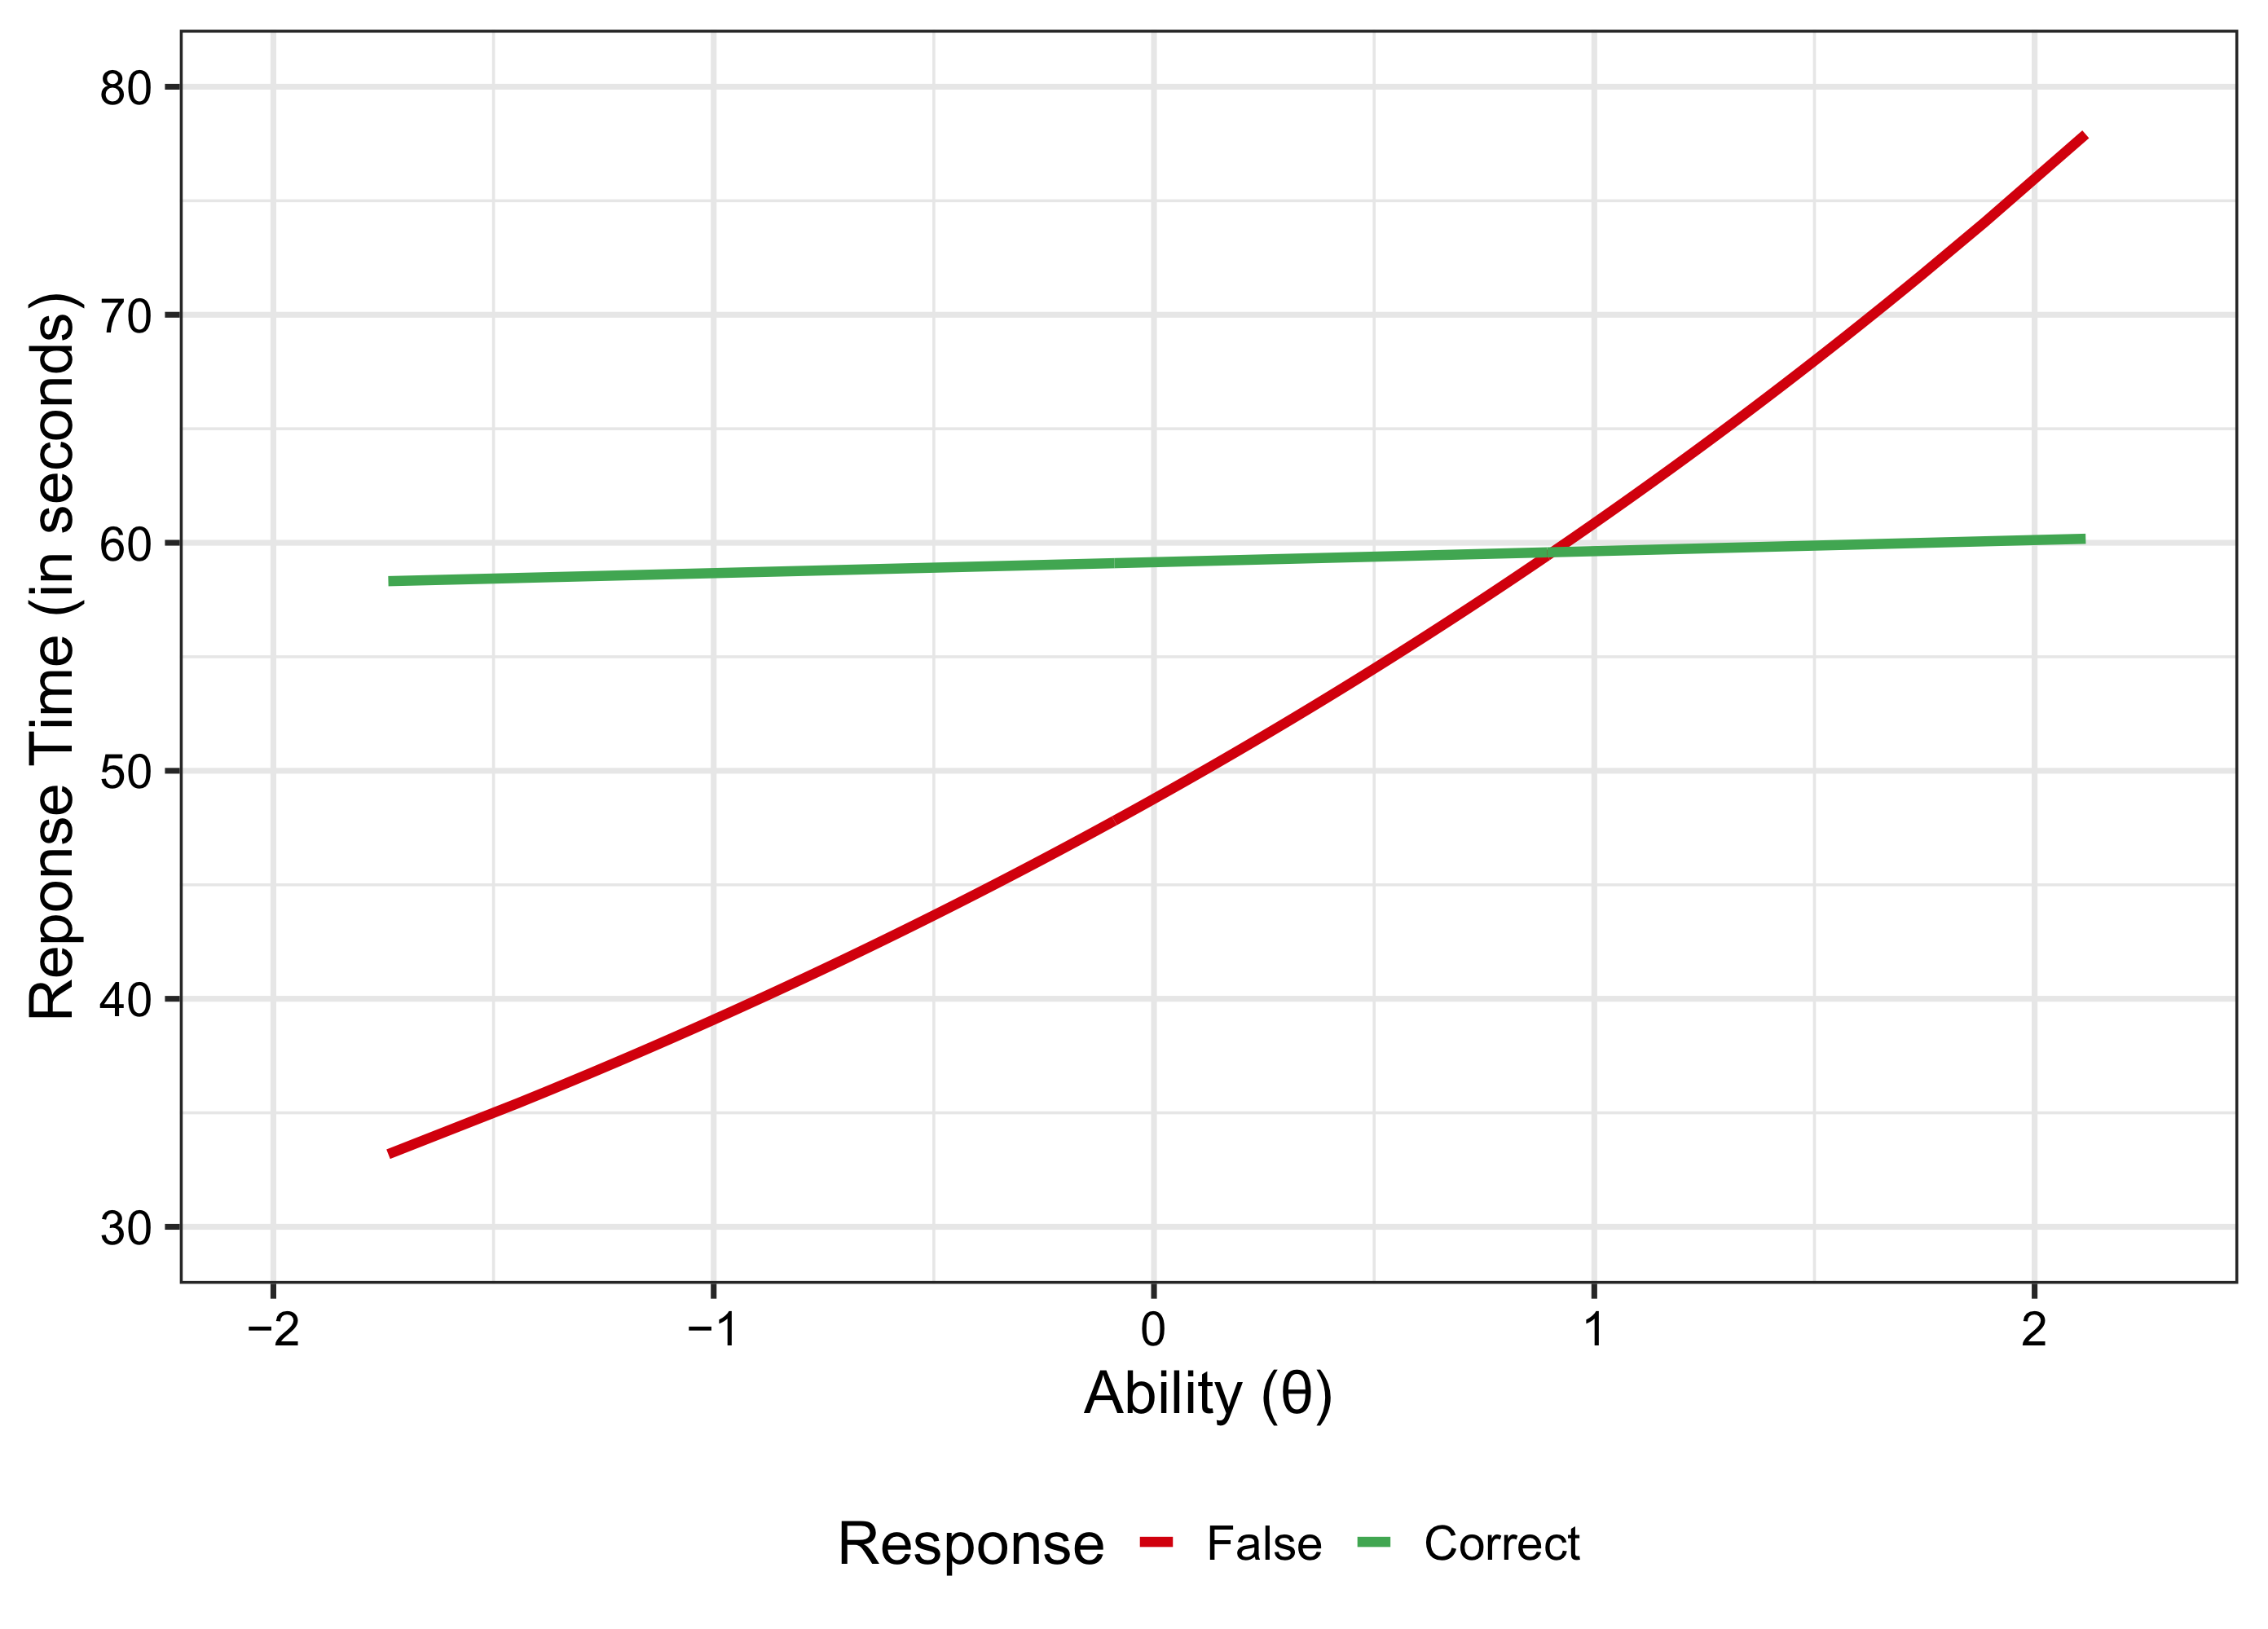
\includegraphics[keepaspectratio]{images/Figure1.png}}

}

\end{figure}%

\begin{figure}

\caption{\label{fig-Figure2}From Model B3, students' predicted response
time according to the discrimination-adjusted ability-difficulty
distance and whether the student answered the question correctly.}

\centering{

\pandocbounded{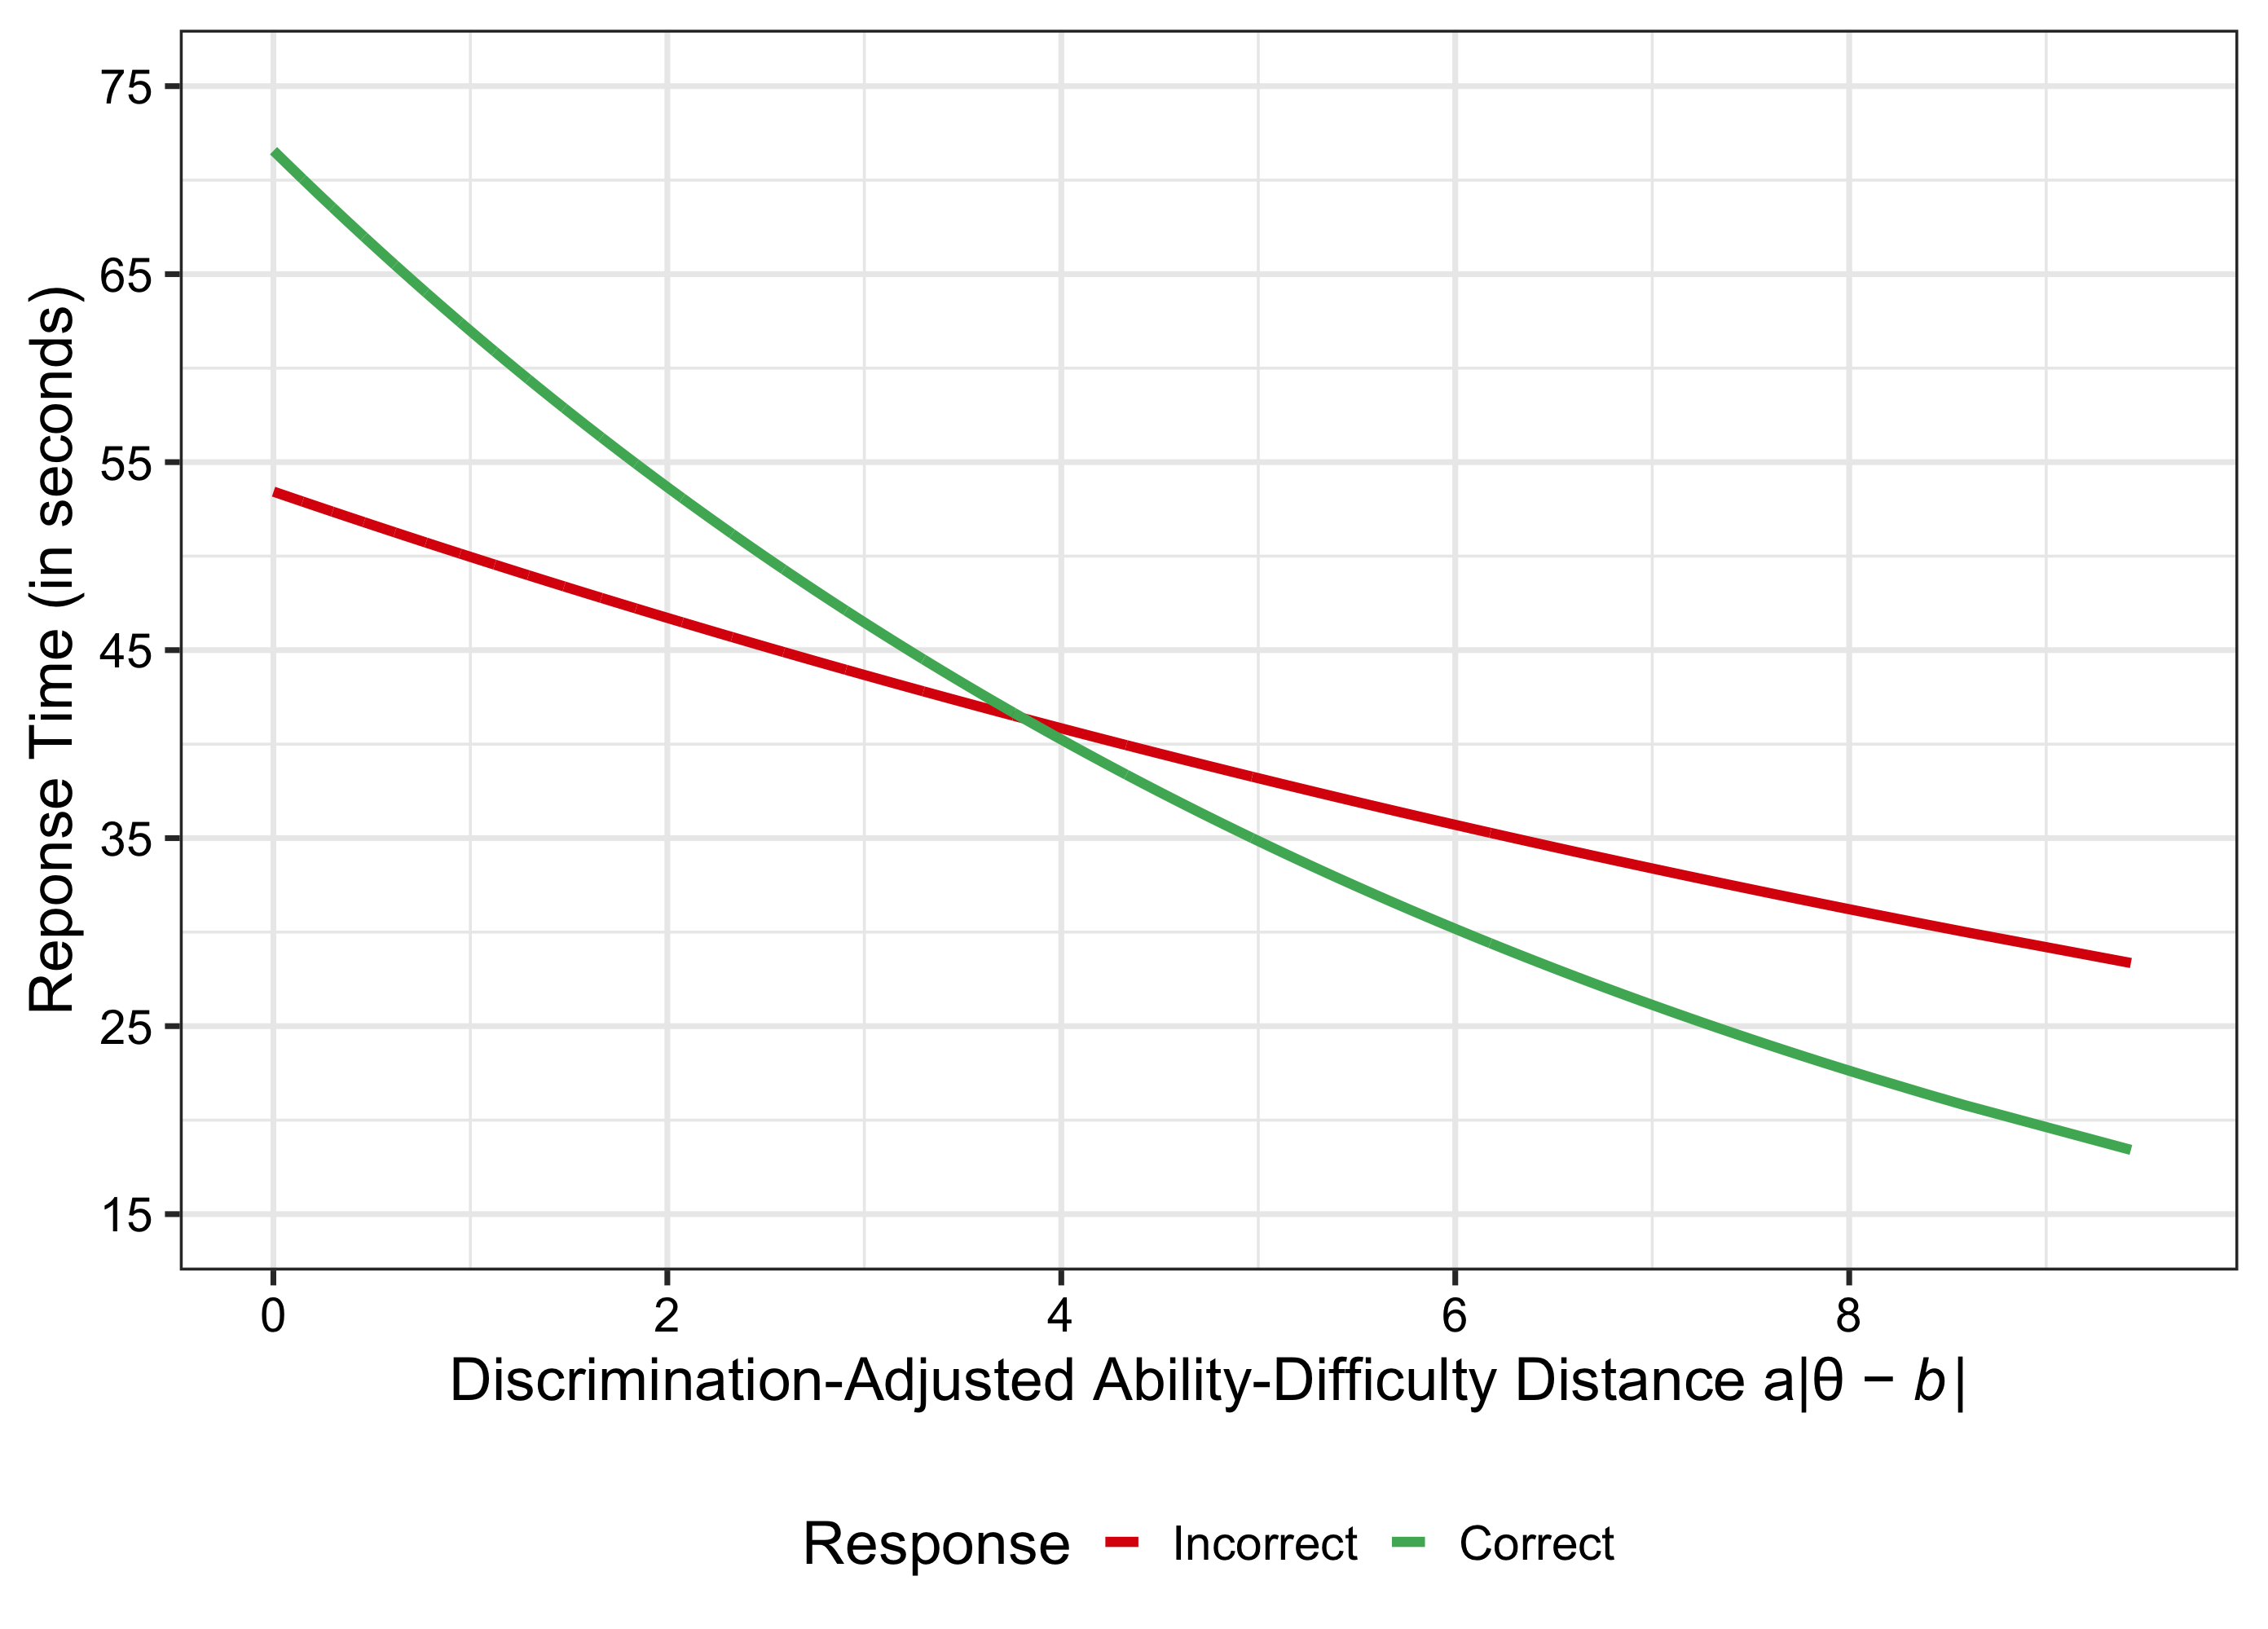
\includegraphics[keepaspectratio]{images/Figure2.png}}

}

\end{figure}%

\section*{Appendix}\label{appendix}
\addcontentsline{toc}{section}{Appendix}

\subsection*{Appendix 1. List of Models
Used}\label{appendix-1.-list-of-models-used}
\addcontentsline{toc}{subsection}{Appendix 1. List of Models Used}

Null Model (Model 0):

\[
\ln{(t_{ij})} = \mu + \nu_j + \beta_i + \epsilon_{ij}
\]

Model A1:

\[
\ln{(t_{ij})} = \mu + \nu_j + \beta_i + \gamma_1 FC_{ij} + \epsilon_{ij}
\]

Model A2:

\[
\ln{(t_{ij})} = \mu + \nu_j + \beta_i + \gamma_1 FC_{ij} + \gamma_2b_i + \gamma_3 \theta_j + \epsilon_{ij}
\]

Model A3:

\[
\ln{(t_{ij})} = \mu + \nu_j + \beta_i + \gamma_1 FC_{ij} + \gamma_2b_i + \gamma_3 \theta_j + \gamma_{13} FC_{ij} \theta_j+ \epsilon_{ij}
\]

Model B1:

\begin{align}
\ln{(t_{ij})} &= \mu + \nu_j + \beta_i + \gamma_4 a_i |\theta_j - b_i|+ \epsilon_{ij} \\
&=\mu + \nu_j +\beta_i +\gamma_4\delta_{ij}+\epsilon_{ij}
\end{align}

Model B2:

\begin{align}
\ln{(t_{ij})} &= \mu + \nu_j + \beta_i + \gamma_4 a_i |\theta_j - b_i|+ \gamma_1FC_{ij}+\epsilon_{ij} \\
&=\mu + \nu_j +\beta_i +\gamma_4\delta_{ij}+\gamma_1 FC_{ij}+\epsilon_{ij}
\end{align}

Model B3:

\begin{align}
\ln{(t_{ij})} &= \mu + \nu_j + \beta_i + \gamma_4 a_i |\theta_j - b_i|+ \gamma_1FC_{ij}+\gamma_{14}FC_{ij}a_i|\theta_j-b_i|+\epsilon_{ij} \\
&=\mu + \nu_j +\beta_i +\gamma_4\delta_{ij}+\gamma_1 FC_{ij}+\gamma_{14}FC_{ij}\delta_{ij}+\epsilon_{ij}
\end{align}

\subsection*{Appendix 2. Booklet Overview for 2019 TIMSS Mathematics
Achievement
Assessment}\label{appendix-2.-booklet-overview-for-2019-timss-mathematics-achievement-assessment}
\addcontentsline{toc}{subsection}{Appendix 2. Booklet Overview for 2019
TIMSS Mathematics Achievement Assessment}

\begin{longtable}[]{@{}lcc@{}}
\toprule\noalign{}
Booklet Number & Isolated Items & Sample Size \\
\midrule\noalign{}
\endhead
\bottomrule\noalign{}
\endlastfoot
1 & 10 & 624 \\
2 & 12 & 621 \\
3 & 12 & 626 \\
4 & 5 & 606 \\
5 & 12 & 619 \\
6 & 11 & 633 \\
7 & 12 & 623 \\
8 & 8 & 617 \\
9 & 11 & 606 \\
10 & 13 & 619 \\
11 & 13 & 620 \\
12 & 11 & 625 \\
13 & 10 & 637 \\
14 & 13 & 622 \\
\end{longtable}

\emph{Note.} Isolated items refer to items that are shown on a webpage
as a stand-alone item. Adapted from Trends in International Mathematics
and Science Study -- TIMSS 2019. Copyright 2021 by International
Association for the Evaluation of Education Achievement (IEA).
Publisher: TIMSS \& PIRLS International Study Center, Lynch School of
Education and Human Development, Boston College.


\nocite{*}



\end{document}
